\documentclass[a4paper]{article}
\usepackage[14pt]{extsizes}
\usepackage[utf8]{inputenc}
\usepackage[russian]{babel}
\usepackage[left=20mm, top=15mm, right=15mm, bottom=15mm, nohead, footskip=10mm]{geometry}
\usepackage{graphicx}

\begin{document}
    \thispagestyle{empty}

    \begin{center}
        Министерство науки и высшего образования Российской Федерации

        Федеральное государственное автономное образовательное учреждение высшего образования

        <<Омский государственный технический университет>>

        \vspace{1cm}
        Факультет информационных технологий и компьютерных систем

        Кафедра <<Прикладная математика и фундаметральная информатика>>

        \vspace{3cm}
        \textbf{Лабораторная работа}

        по дисциплине <<Теория вероятностей и математическая статистика>>
    \end{center}
    
    \vspace{3cm}
    \begin{flushright}    
        \begin{tabular}{ r r }
            Студента & Курпенова Куата Ибраимовича \\
            \cline{2-2}
            & \tiny{фамилия, имя, отчество полностью} \\

            Курс & 3, группа ФИТ-222 \\
            \cline{2-2}
            Направление & 02.03.02 Прикладная математика \\
            \cline{2-2}
            & и фундаментальная информатика \\
            \cline{2-2}
            & \tiny{код, наименование} \\
            
            Руководитель & доц., канд. тех. наук \\
            \cline{2-2}
            & \tiny{должность, ученая степень, звание} \\
            & Болдовская Т. Е. \\
            \cline{2-2}
            & \tiny{фамилия, инициалы} \\
            
            Выполнил & \\
            \cline{2-2}
            & \tiny{дата, подпись студента} \\
            
        \end{tabular}
    \end{flushright}
    
    \vspace*{\fill}
    \begin{center}
        Омск 2024
    \end{center}

    \newpage

    \section*{Проверка гипотезы о законе распределения генеральной совокупности}

    \subsection*{Данные из выборки}
    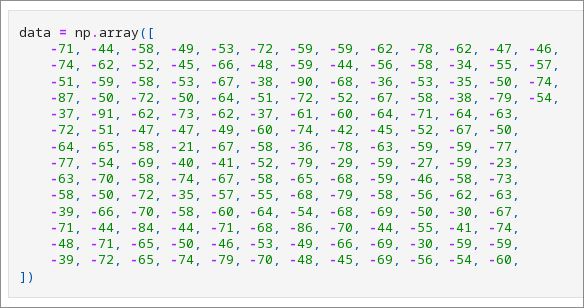
\includegraphics[width=\textwidth]{images/data.png}

    \subsection*{Вариационный ряд}
    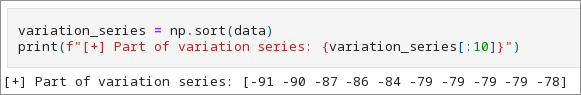
\includegraphics[width=\textwidth]{images/variation_series.png}

    \subsection*{Интервальный статистический ряд}
    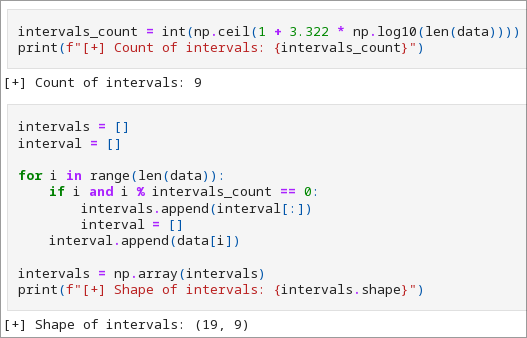
\includegraphics[width=\textwidth]{images/interval_series.png}

    \subsection*{Полигон и гистограмма относительных частот}
    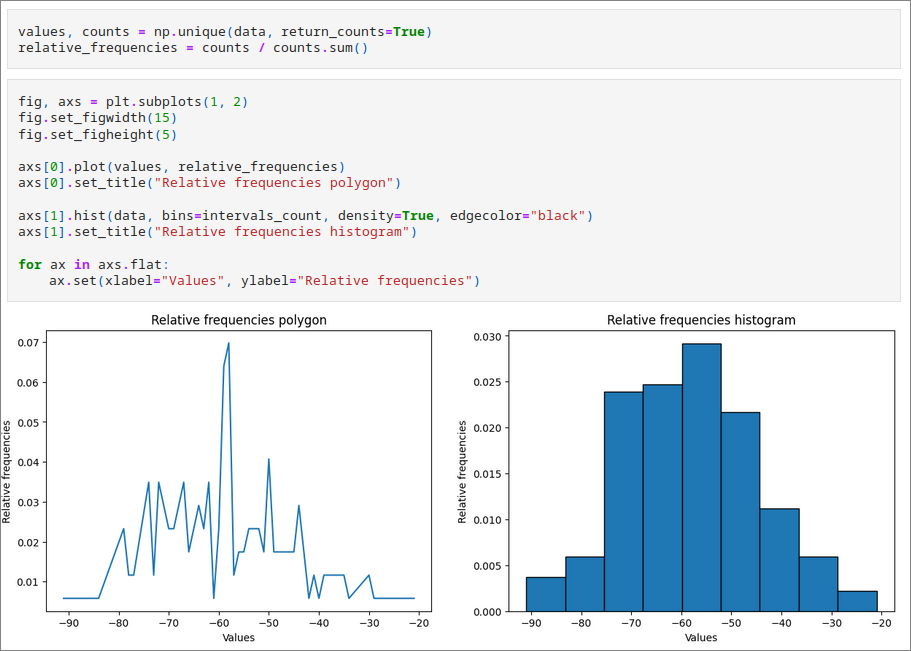
\includegraphics[width=\textwidth]{images/relative_frequencies.png}

    \subsection*{График эмпирической функции распределения}
    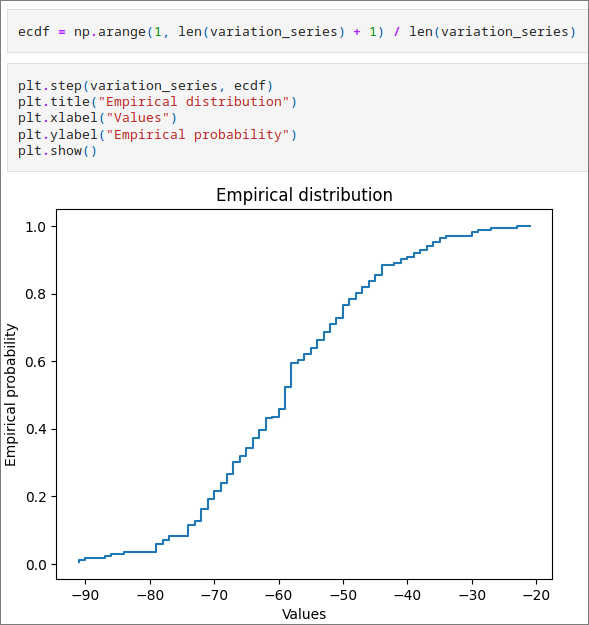
\includegraphics[width=\textwidth]{images/empirical_distribution.png}

    \subsection*{Числовые характеристики выборки}
    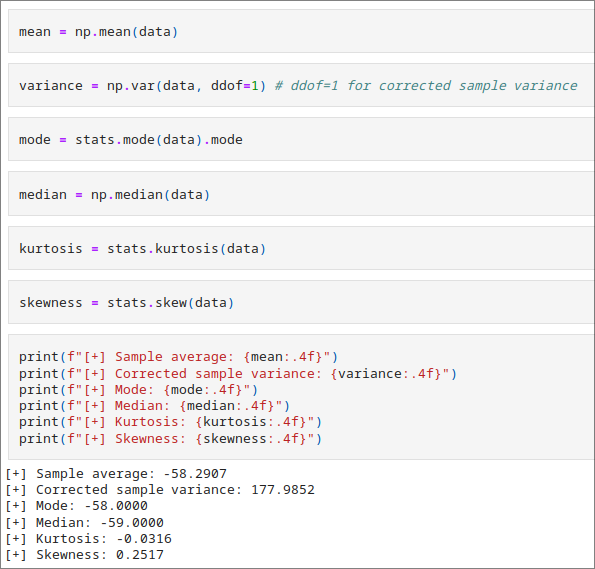
\includegraphics[width=\textwidth]{images/characteristics.png}

    \subsection*{Гипотеза о распределении генеральной совокупности}

    Я предполагаю, что распределение является нормальным, так как гистограмма относительных частот похожа на нормальное распределение, а график эмпирического распределения похож на сигмоиду.

    \subsection*{Оценка параметров нормального распределения генеральной совокупности}
    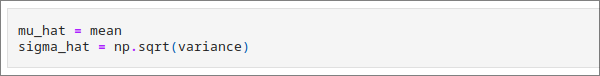
\includegraphics[width=\textwidth]{images/assessment.png}

    \subsection*{Теоретические аналоги функции}
    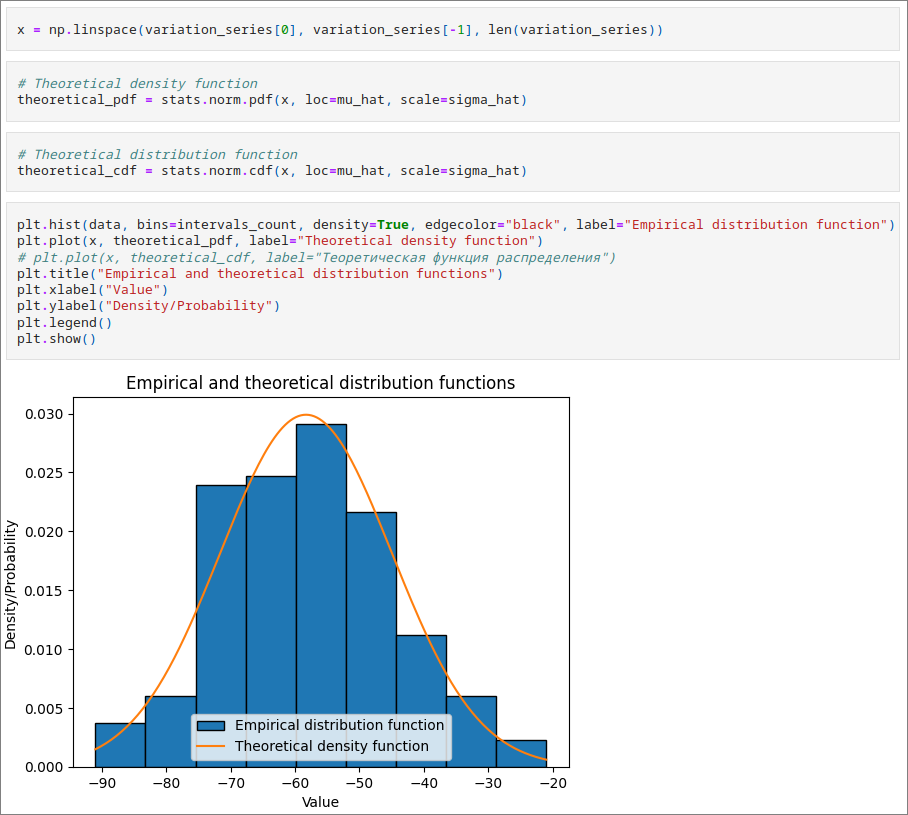
\includegraphics[width=\textwidth]{images/theoretical_analogs.png}
    
    \subsection*{Выполнение правила "трёх сигма"}
    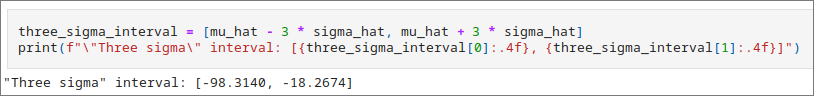
\includegraphics[width=\textwidth]{images/three_sigma.png}

    \subsection*{Проверка по критерию Пирсона}
    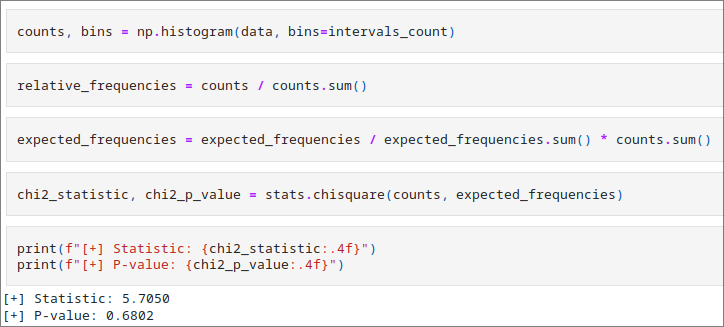
\includegraphics[width=\textwidth]{images/pearson.png}

    \subsection*{Проверка по критерию Колмогорова}
    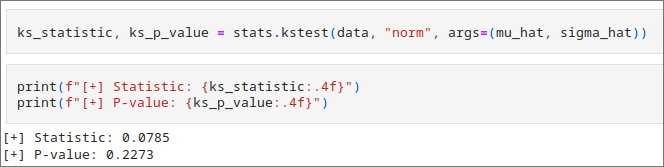
\includegraphics[width=\textwidth]{images/kolmogorov.png}

    \subsection*{Построение доверительного интервала}
    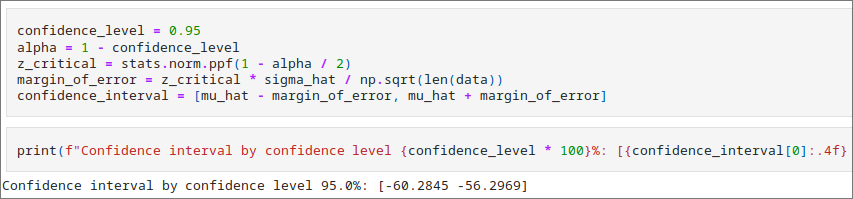
\includegraphics[width=\textwidth]{images/confidence_interval.png} 

\end{document}
